\documentclass[11pt]{article}
\usepackage{../EllioStyle}
\usepackage{listings}
\usepackage{multicol}
\usepackage{forest}

\definecolor{codegreen}{rgb}{0,0.6,0}
\definecolor{codegray}{rgb}{0.5,0.5,0.5}
\definecolor{codepurple}{rgb}{0.58,0,0.82}
\definecolor{backcolour}{rgb}{0.95,0.95,0.92}

\lstdefinestyle{mystyle}{
%    backgroundcolor=\color{backcolour},   
    commentstyle=\color{codegreen},
    keywordstyle=\color{magenta},
    numberstyle=\tiny\color{codegray},
    stringstyle=\color{codepurple},
    basicstyle=\ttfamily\footnotesize,
    breakatwhitespace=false,         
    breaklines=true,                 
    captionpos=b,                    
    keepspaces=true,                 
    numbers=left,                    
    numbersep=5pt,                  
    showspaces=false,                
    showstringspaces=false,
    showtabs=false,                  
    tabsize=2
}

\title{Homework 4}
\author{Elliott Pryor}
\date{14 November 2021}

\rhead{Homework 4}

\begin{document}
\maketitle

\problem{1}
Consider the follwing set of sequences:

\begin{align*}
    S_1 &= ACTCTCGATC\\
    S_2 &= ACTTCGATC \\
    S_3 &= ACTCTCTATC \\
    S_4 &= ACTCTCTAATC
\end{align*}

Compute the MSA using the center star method.

\hrule

We give the pairwise distances

\begin{table}[H]
    \centering
    \begin{tabular}{c | c | c | c | c }
              & $S_1$ & $S_2$ & $S_3$ & $S_4$ \\ \hline
        $S_1$ &  0    &  1    &   1   & 2     \\ \hline
        $S_2$ & 1     &   0   &   2   & 3     \\ \hline
        $S_3$ &  1    &   2   &   0   & 1     \\ \hline
        $S_4$ &  2    &   3   &  1    & 0     \\ \hline
        
    \end{tabular}
\end{table}

We get that $S_1$ or $S_3$ would be equally good center stars. 
We pick $S_1$.

\begin{multicols}{2}

We compute alignments with $S_1$:

\begin{align*}
    S_1 &= ACTCTCGATC\\
     &= ACTCTCGATC \\
    S_2 &= ACTCTCGATC \\
    &= ACT\_TCGATC \\
    S_3 &= ACTCTCGATC \\
    &= ACTCTCTATC \\
    S_4 &= ACTCTCG\_ATC \\
    &= ACTCTCTAATC \\
\end{align*}

\columnbreak

From this we get the MSA:

\begin{align*}
    &ACTCTCG\_ \; ATC \\
    &ACT\_ \; TCG\_ \; ATC \\
    &ACTCTCT\_ \; ATC \\
    &ACTCTCTAATC \\
\end{align*}

\end{multicols}


\problem{2}
Compute the ClustalW alignment of the previous problem:

\hrule


\begin{table}[H]
    \centering
    \begin{tabular}{c | c | c | c | c }
              & $S_1$ & $S_2$ & $S_3$ & $S_4$ \\ \hline
        $S_1$ &  0    &   0   &   0.1   & 0.1     \\ \hline
        $S_2$ &  0    &   0   &   $\bar{0.1}$   & $\bar{0.1}$     \\ \hline
        $S_3$ &  0    &   0   &   0   & 0     \\ \hline
        $S_4$ &  0    &   0   &   0   & 0     \\ \hline
        
    \end{tabular}
\end{table}

\begin{figure}[h] 
    \centering
    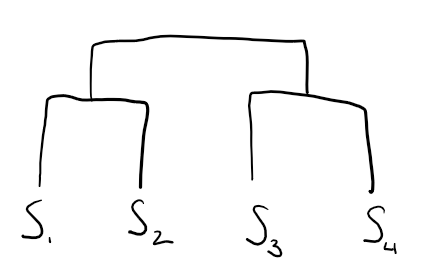
\includegraphics[width=0.55 \linewidth]{tree.png}
    \label{fig:}
    \caption{Guide tree}
\end{figure}

Aligning $S_1, S_2$ produces ($ACTCTCGATC, ACT\_ \; TCGATC$),

aligning $S_3, S_4$ produces ($ACTCTCT\_ \; ATC, ACTCTCTAATC$).

Then using the profile-profile alignment we get:

\begin{align*}
    &ACTCTCGATC\_  \\
    &ACT\_ \; TCGATC\_ \\
    &ACTCTCTATC \_ \\
    &ACTCTCTAATC
\end{align*}


\problem{3}
Given a set of $k$ sequences: $S_1, \dots , S_k$ find $k$ substrings such that the optimal SP score of multiple sequence alignment is maximized.
Give a Dynamic Programming algorithm to solve this. (Note, when $k=2$ this is same as solving local alignment problem)

\hrule

We build a generalized version of Smith-Waterman algorithm.
We base this on the generalized verson of Needleman-Wunch algorithm from class:
$$V(i_1, \dots, i_k) = \max _{b_1, \dots, b_k \in \{(0,1)\}^k \setminus (0,0) } V(i_1 - b_1, \dots, i_k - b_k) + SP(S_1[i_1 b_1], \dots S_k[i_k b_k])$$

We note that the only difference in the Smith-Waterman algorith from the Needleman-Wunch algorithm is the option to take a score of 0 always.
So we have a generalized Smith-Waterman:
$$V(i_1, \dots, i_k) = \max _{b_1, \dots, b_k \in \{(0,1)\}^k \setminus (0,0) } (V(i_1 - b_1, \dots, i_k - b_k) + SP(S_1[i_1 b_1], \dots S_k[i_k b_k]), 0)$$

With a base case of $V(0, \dots, 0) = 0$ and $i_j = 0 \implies b_j = 0$.

Then we have to find the local alignment with the best score. This is the entry with the greatest value in the matrix.
So the optimal score is $max_{i_1 \dots i_k} V(i_1 \dots i_k)$.

Building the matrix $V$ takes $O(n^k)$ space. For running time we have $O(n^k)$ entries to fill out, $2^k - 1$ options for $b$, and $k \choose 2$ evaluations of $SP$.
Thus we have $O(n^k 2^k k^2)$ time (same as generalized Needleman-Wunch) to build $V$.
Then we need to find the max in $V$: which is just searching through all $n^k$ entries.
Thus our running time is: $O(n^k 2^k k^2)$

\problem{4}
Code Center Star Algorithm.

\hrule


\begin{figure}[h] 
    \centering
    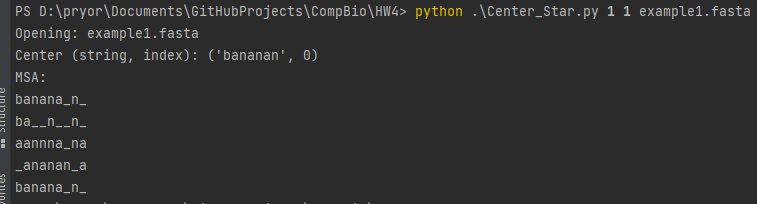
\includegraphics[width=0.55 \linewidth]{example1.png}
    \label{fig:}
    \caption{Example showing execution on example1}
\end{figure}

\begin{figure}[h] 
    \centering
    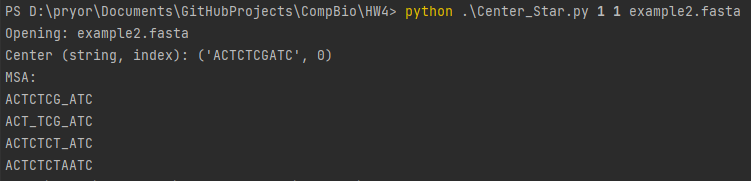
\includegraphics[width=0.55 \linewidth]{example2.png}
    \label{fig:}
    \caption{Example showing execution on strings from Problem 1}
\end{figure}

\lstinputlisting{example1.fasta}
\lstinputlisting{example2.fasta}

\lstset{style=mystyle}
\lstinputlisting[language=Python]{Center_Star.py}


\end{document}